\section{Capacitancia y materiales dieléctricos}
  \subsection{Definición de capacitancia}
    \PN La combinación de dos conductores se conoce como \textbf{capacitor}. Los conductores son las placas. Si los
    conductores llevan carga de igual magnitud y signo opuesto existe una diferencia de potencial $\Delta V$ entre
    ellos.

    \VS
    \PN La cantidad de carga Q en un capacitor es linealmente proporcional a la diferencia de potencial entre los
    conductores; es decir, $Q \propto V$. La constante de proporcionalidad depende de la forma y separación de los
    conductores. Esta relación se escribe como $Q = C \Delta V$ si define la capacitancia de la siguiente manera:

    \VS
    \PN \textbf{Definición:} La \textbf{capacitancia} $C$ de un capacitor se define como la relación de la magnitud de
    la carga en cualquiera de los conductores a la magnitud de la diferencia de potencial entre dichos conductores:
    \begin{equation*}
      C \equiv \frac{Q}{\Delta V}
    \end{equation*}

    \PN La capacitancia siempre es una cantidad positiva. Además, la carga $Q$ y la diferencia de potencial $\Delta V$
    siempre se expresan como cantidades positivas.

    \VS
    \PN En unidades del SI la capacitancia se expresa en coulombs por cada volt. La unidad del SI para capacitancia es
    el \textit{farad} (F).
    \begin{equation*}
      1 \ \text{F} = 1 \ \frac{\text{C}}{\text{V}}
    \end{equation*}

    \PN Piense en un capacitor formado por un par de placas paralelas, cada placa está conectada a una de las terminales
    de una batería, que actúa como fuente de diferencia de potencial. Si al inicio el capacitor no está cargado, la
    batería establece una campo eléctrico en los alambres de conexión cuando se cierra el circuito. La diferencia de
    potencial entre las capas del capacitor es la misma que existe entre las terminales de la batería.

  \subsection{Cálculo de la capacitancia}
    \PN Es posible deducir una expresión para la capacitancia producida por un par de conductores de cargas opuestas con
    una carga de magnitud $Q$, de la siguiente manera: primero calcule la diferencia de potencial. A continuación
    utilice la expresión $C = Q / \Delta V$ a fin de evaluar la capacitancia.
    \PN Sin embargo, la situación más común es que de dos conductores, solo un conductor también tenga capacitancia. Por
    ejemplo, imagine un conductor esférico con carga. Las líneas del campo eléctrico alrededor de este conductor son
    exactamente las mismas que si se tratara de una cubierta conductora, esférica de radio infinito, concéntrico con la
    esfera, y con una carga de la misma magnitud pero de signo opuesto. Por lo tanto, identifique esta cubierta
    imaginaria como el segundo conductor de un capacitor de dos conductores. El potencial eléctrico de una esfera de
    radio r es simplemente $k Q/a$, y si $V = 0$ en el caso de la cubierta infinitamente grande, tiene
    \begin{equation*}
      C = \frac{Q}{\Delta V} = \frac{Q}{k Q/a} = \frac{r}{k} = 4 \pi \epsilon_{0} r
    \end{equation*}

    \PN Esta expresión muestra que la capacitancia de una esfera con carga y aislada es proporcional a su radio y es
    independiente tanto de la carga de la esfera como de la diferencia de potencial.

    \PN La capacitancia de un par de conductores se ilustra mediante tres geometrías comunes, sobre todo, placas
    paralelas, cilindros concéntricos y esferas concéntricas. En estos ejemplos, suponga que los conductores cargados
    están separados por un espacio vacío.

    \subsubsection{Capacitor de placas paralelas}
      \PN Dos placas metálicas paralelas de igual área $A$ están separadas por una distancia $d$. Una placa tiene una
      carga $+Q$ y la otra tiene una carga $–Q$. La densidad de carga superficial en cada placa es $ \sigma = Q/A$. El
      valor del campo eléctrico entre las placas es
      \begin{equation*}
        E = \frac{\sigma}{\epsilon_{0}} = \frac{Q}{\epsilon_{0}A}
      \end{equation*}

      \PN Ya que el campo entre las placas es uniforme, la magnitud de la diferencia de potencial entre las placas es
      igual a Ed, por lo tanto
      \begin{equation*}
        \Delta V = Ed = \frac{Qd}{\epsilon_{0}A}
      \end{equation*}

      \PN Luego, la capacitancia es
      \begin{equation*}
        C = \frac{Q}{\Delta V} = \frac{Q}{Qd/\epsilon_{0}A} = \frac{\epsilon_{0}A}{d}
      \end{equation*}

      \PN Es decir, la capacitancia de un capacitor de placas paralelas es proporcional al área de sus placas e
      inversamente proporcional a la separación de las placas.

  \subsection{Combinaciones de capacitores}
    \PN En los circuitos eléctricos con frecuencia se combinan dos o más capacitores. Es posible calcular la
    capacitancia equivalente de ciertas combinaciones, en donde supondrá que los capacitores a combinar están
    inicialmente descargados.

    \subsubsection{Combinación en paralelo}
      \begin{figure}[H]
      \centering
        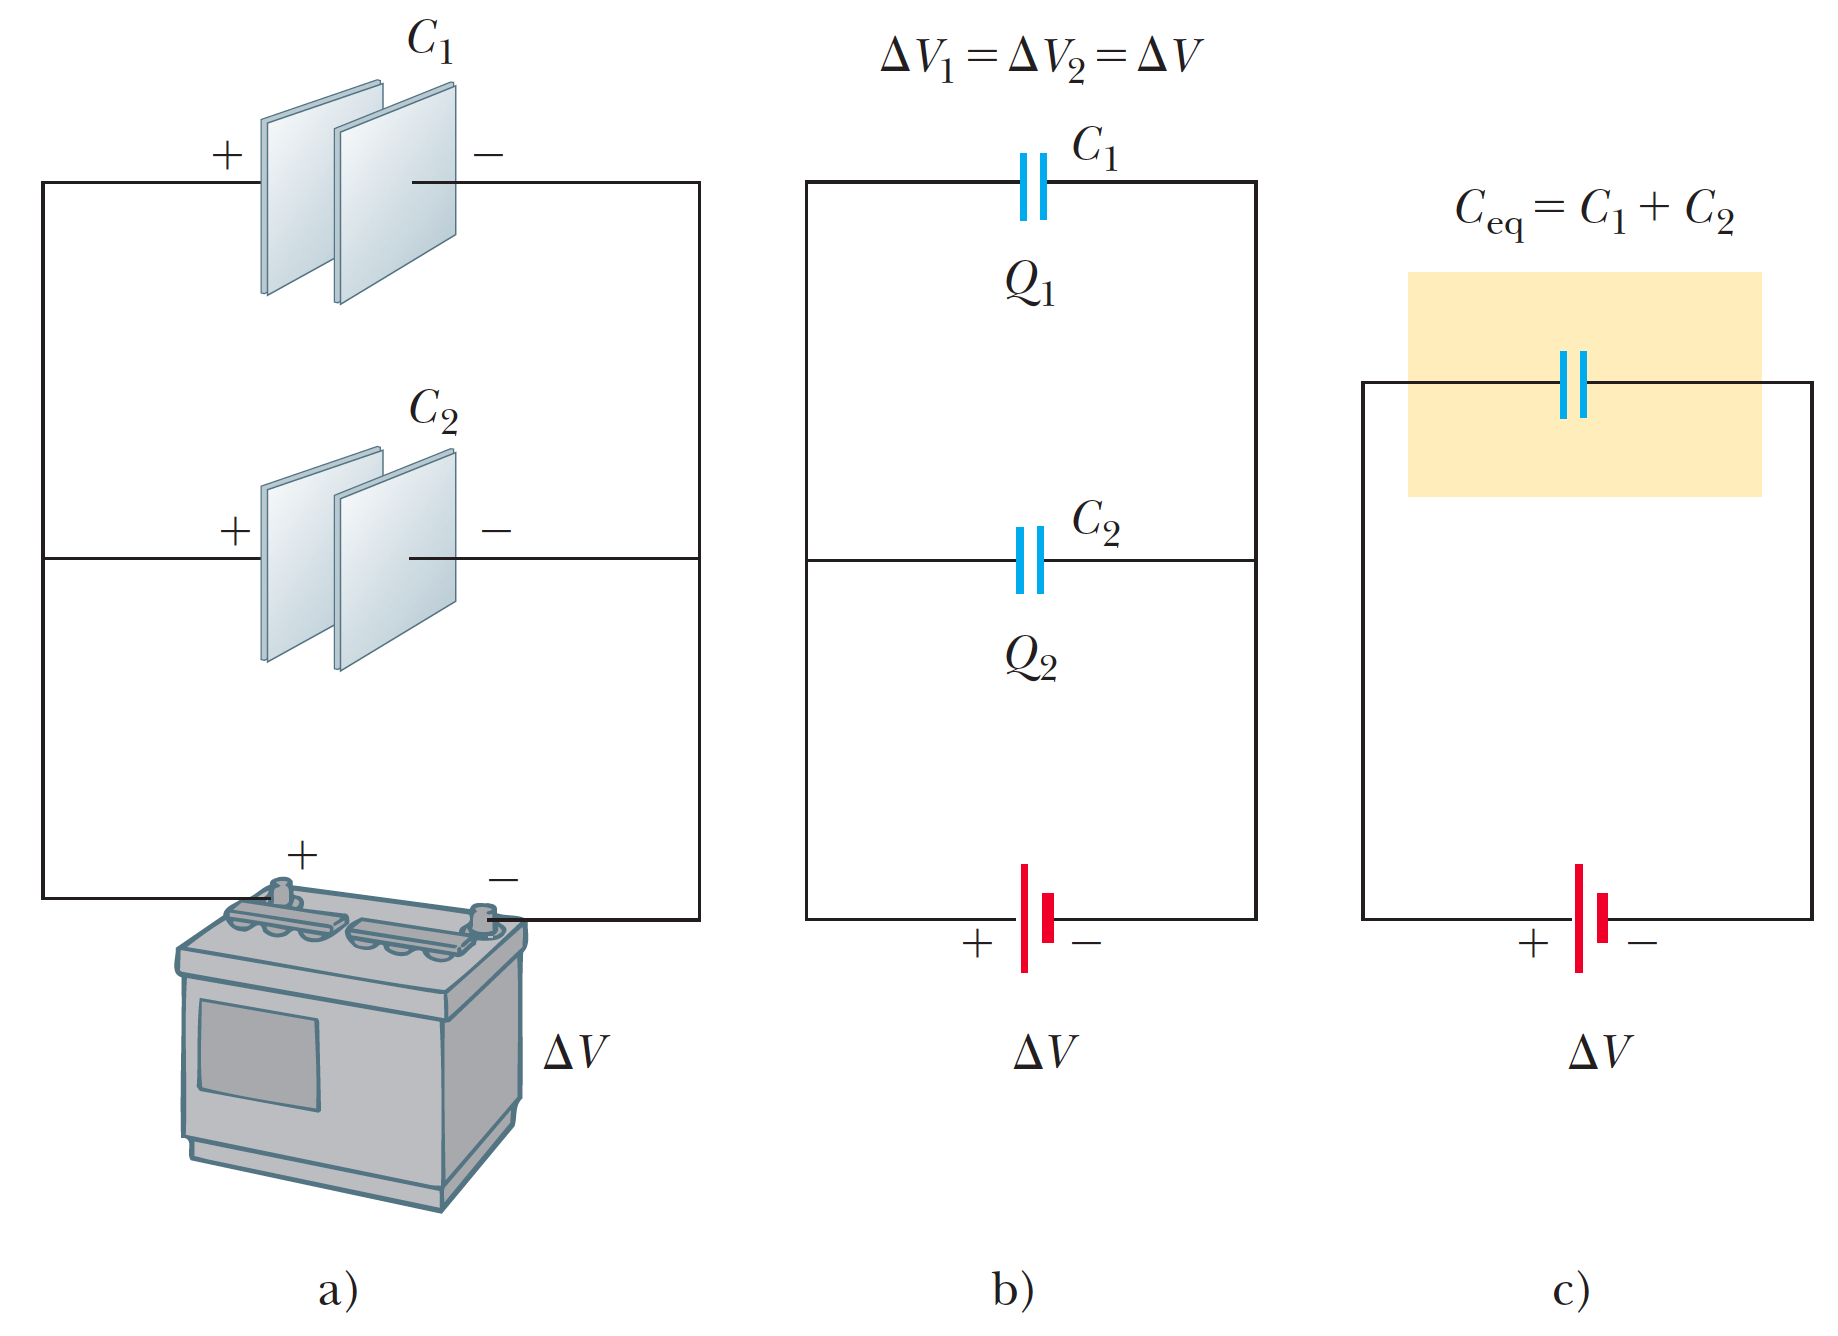
\includegraphics[width=0.55\textwidth]{4/figure_6}
        \caption{a) Una combinación en paralelo de dos capacitores en un circuito eléctrico en el cual la diferencia de
        potencial entre las terminales de la batería, es igual a V. b) Diagrama de circuito para esta combinación en
        paralelo. c) La capacitancia equivalente.}
      \end{figure}

      \PN Las diferencias de potencial individuales a través de capacitores conectados en paralelo son las mismas e
      iguales a la diferencia de potencial aplicada a través de la combinación. Es decir,
      \begin{equation*}
        \Delta V = \Delta V_{1} = \Delta V_{2}
      \end{equation*}

      \PN donde $\Delta V$ es el voltaje de terminal de la batería.

      \VS
      \PN Después de que la batería se une al circuito, los capacitores rápidamente alcanzan su carga máxima. Sean las
      cargas máximas en los dos capacitores $Q_{1}$ y $Q_{2}$. La carga total $Q_{tot}$ almacenada por los dos
      capacitores es
      \begin{equation*}
        Q_{tot} = Q_{1} + A_{2}
      \end{equation*}

      \PN Es decir, la carga total en capacitores conectados en paralelo es la suma de las cargas en los capacitores
      individuales.

      \VS
      \PN Suponga que quiere sustituir estos dos capacitores por un capacitor equivalente que tenga una capacitancia
      $C_{eq}$. El efecto que este capacitor equivalente tiene sobre el circuito debe ser exactamente el mismo que el
      efecto de la combinación de los dos capacitores individuales. Es decir: el capacitor equivalente debe almacenar
      carga $Q_{tot}$ cuando se conecte a la batería. El voltaje a través del capacitor equivalente es $\Delta V$ porque
      el capacitor equivalente se conecta directamente a través de las terminales de la batería. Por lo tanto, para el
      capacitor equivalente,
      \begin{equation*}
        Q_{tot} = C_{eq} \ \Delta V
      \end{equation*}

      \PN Luego
      \begin{eqnarray*}
        C_{eq} \ \Delta V = C_{1} \ \Delta V_{1} = C_{2} \ \Delta V_{2} \\
        C_{eq} = C_{1} + C_{2} \ \text{(combinaciones en paralelo)}
      \end{eqnarray*}

      \PN donde se cancelan los voltajes porque todos son iguales. Si este tratamiento se extiende a tres o más
      capacitores conectados en paralelo, se encuentra que la capacitancia equivalente
      \begin{equation*}
        C_{eq} = C_{1} + C_{2} + \dotsc \ \text{(combinaciones en paralelo)}
      \end{equation*}

    \subsubsection{Combinación en serie}
      \begin{figure}[H]
      \centering
        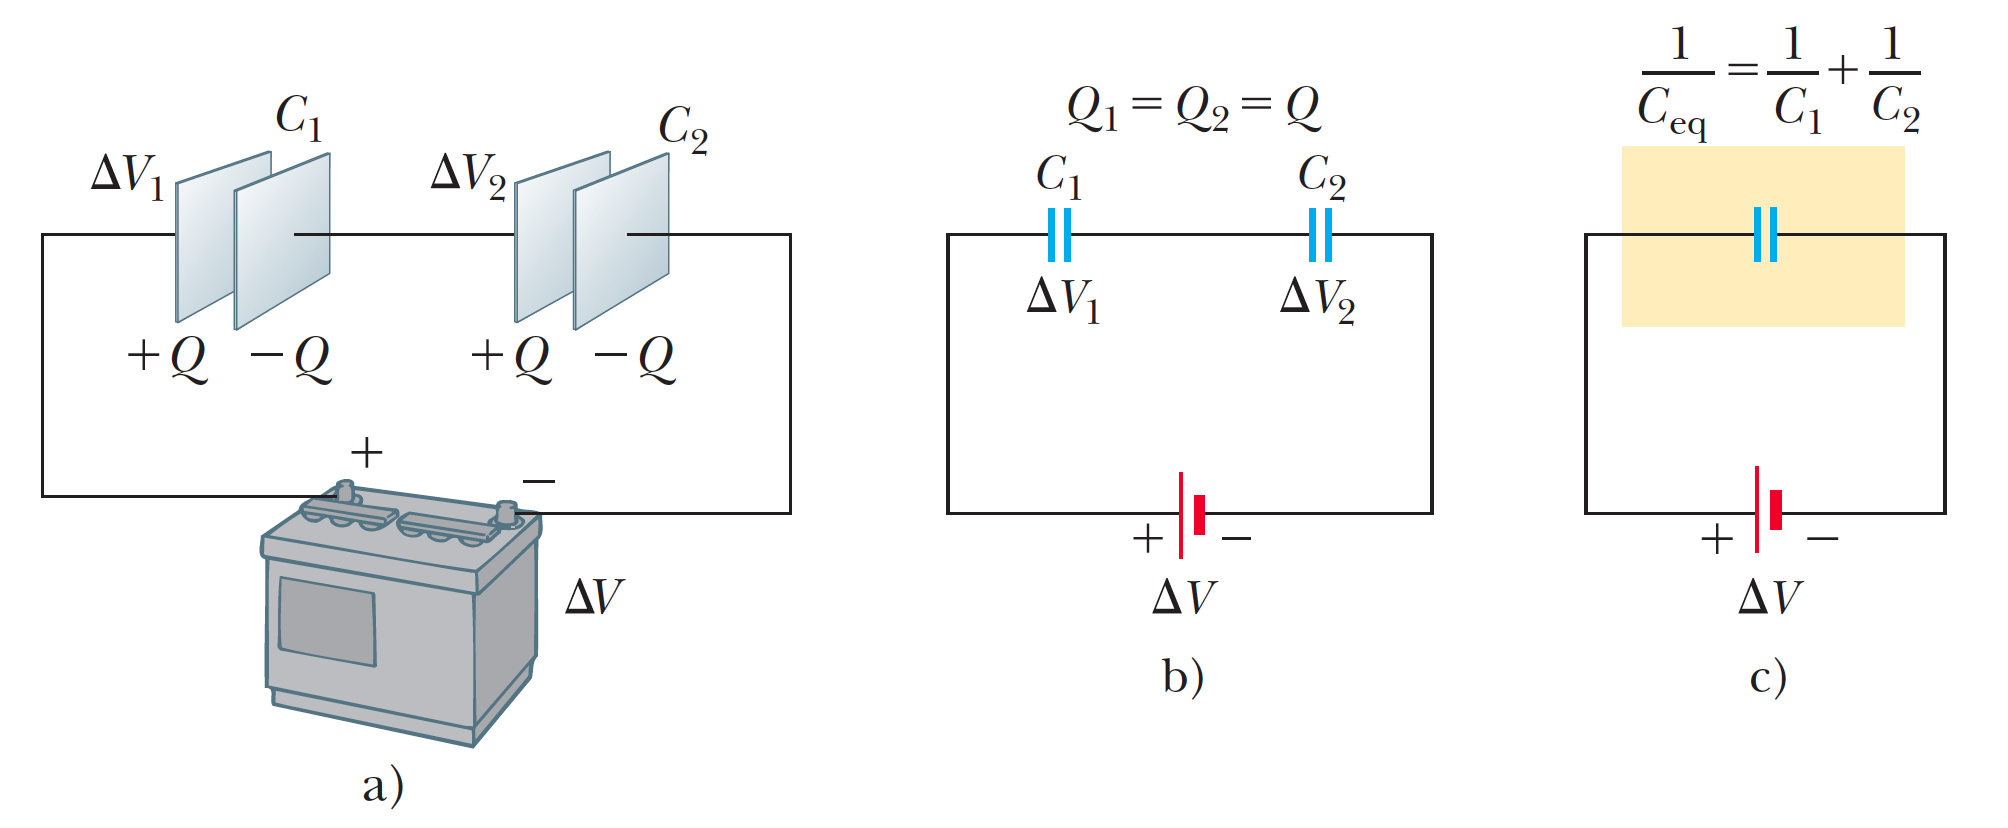
\includegraphics[width=0.7\textwidth]{4/figure_7}
        \caption{a) Combinación en serie de dos capacitores. Las cargas en ambos capacitores son iguales. b) Diagrama
        del circuito para la combinación en serie. c) La capacitancia equivalente.}
      \end{figure}

      \PN Las cargas de los capacitores conectados en serie son iguales.
      \begin{equation*}
        Q = Q_{1} = Q_{2}
      \end{equation*}

      \PN donde $Q$ es la carga que se movió entre un alambre y la placa exterior conectada de uno de los capacitores.

      \PN El voltaje total $V_{tot}$ a través de la combinación se divide entre los dos capacitores:
      \begin{equation*}
        \Delta V_{tot} = \Delta V_{1} + \Delta V_{2}
      \end{equation*}

      \PN donde $V_{1}$ y $V_{2}$ son las diferencias de potencial presentes en los capacitores $C_{1}$ y $C_{2}$,
      respectivamente. En general, la diferencia de potencial total aplicada a cualquier cantidad de capacitores
      conectados en serie es la suma de las diferencias de potencial presentes entre cada uno de los capacitores
      individuales.

      \VS
      \PN Suponga que el simple capacitor individual equivalente ejerce un efecto idéntico sobre el circuito que la
      combinación en serie cuando está conectado a la batería. Una vez que está totalmente cargado, el capacitor
      equivalente deberá tener una carga igual a $-Q$ en su placa derecha y una carga de $+Q$ en su placa izquierda. Al
      aplicar la definición de capacitancia se tiene
      \begin{eqnarray*}
        \Delta V_{tot} = \frac{Q}{C_{eq}} \\
        \frac{Q}{C_{eq}} = \frac{Q_{1}}{C_{1}} + \frac{Q_{2}}{C_{2}}
      \end{eqnarray*}

      \PN Se cancelan las cargas porque son las mismas
      \begin{equation*}
        \frac{1}{C_{eq}} = \frac{1}{C_{1}} + \frac{1}{C_{2}} \ \text{(combinaciones en serie)}
      \end{equation*}

      \PN Cuando es aplicado este análisis a una combinación de tres o más capacitores conectados en serie, la
      correspondencia para la capacitancia equivalente es
      \begin{equation*}
        \frac{1}{C_{eq}} = \frac{1}{C_{1}} + \frac{1}{C_{2}} + \dotsc \ \text{(combinaciones en serie)}
      \end{equation*}

  \subsection{Energía almacenada en un capacitor con carga}
    \PN Ya que las cargas positiva y negativa están separadas en el sistema de dos conductores en un capacitor, en el
    sistema se almacena energía potencial eléctrica.

    \VS
    \PN Suponga que $q$ es la carga del capacitor en un determinado instante durante el proceso de carga. En ese mismo
    momento, la diferencia de potencial a través del capacitor es $\Delta V = q/C$. Se sabe que el trabajo necesario
    para transferir un incremento de carga $dq$ de la placa que tiene una carga $-q$ a la placa que tiene una carga $+q$
    es
    \begin{equation*}
      dW = \Delta V \ dq = \frac{q}{C} \ dq
    \end{equation*}

    \PN El trabajo total requerido para cargar el capacitor desde $q = 0$ hasta una carga final $q = Q$ es
    \begin{equation*}
      W = \int_{0}^{Q} \frac{q}{C} \ dq = \frac{1}{C} \int_{0}^{Q} q \ dq = \frac{Q^{2}}{2C}
    \end{equation*}

    \PN El trabajo invertido al cargar el capacitor se presenta como una energía potencial eléctrica $U$ almacenada en
    el mismo. Es posible expresar la energía potencial almacenada en el capacitor con carga como:
    \begin{equation*}
      U = \frac{Q^{2}}{2C} = \frac{1}{2} Q \ \Delta V = \frac{1}{2} C (\Delta V)^{2}
    \end{equation*}

    \PN Este resultado es aplicable a cualquier capacitor, sea cual fuere su geometría. Para una capacitancia
    determinada, la energía almacenada aumenta al incrementarse la carga y la diferencia de potencial.

    \VS
    \PN Considere la energía almacenada en un capacitor como si estuviera almacenada en el campo eléctrico producido
    entre las placas al cargar el capacitor. En el caso de un capacitor de placas paralelas, la diferencia de potencial
    está relacionada con el campo eléctrico mediante la correspondencia $\Delta V = Ed$. Además, su capacitancia es
    $C = \epsilon_{0} A/d$. Si sustituyen estas expresiones, se obtiene
    \begin{equation*}
      U = \frac{1}{2} \frac{\epsilon_{0}A}{d} (E^{2}d^{2}) = \frac{1}{2} (\epsilon_{0}Ad) E^{2}
    \end{equation*}

    \PN En vista de que el volumen ocupado por el campo eléctrico es $Ad$, la energía por cada unidad de volumen
    $u_{E} = U/Ad$, conocida como \textit{densidad de energía}, es
    \begin{equation*}
      u_{E} = \frac{1}{2} \epsilon_{0} E^{2}
    \end{equation*}

    \PN Esta expresión es válida de manera general, independientemente de la fuente del campo eléctrico. Es decir, la
    densidad de energía en cualquier campo eléctrico en un punto dado es proporcional al cuadrado de la magnitud del
    campo eléctrico.

  \subsection{Capacitores con material dieléctrico}
    \PN Un \textbf{dieléctrico} es un material no conductor. Consideremos un capacitor de placas paralelas que, sin
    dieléctrico, tiene una carga $Q_{0}$ y una capacitancia $C_{0}$. La diferencia de potencial en las terminales del
    capacitor es $V_{0} = Q_{0}/C_{0}$. Si ahora se inserta un material dieléctrico entre las placas, el voltímetro
    indica que el voltaje entre las placas disminuye un valor $\Delta V$. Los voltajes con y sin dieléctrico están
    relacionados mediante el factor $k$ como sigue:
    \begin{equation*}
      \Delta V = \frac{\Delta V_{0}}{k}
    \end{equation*}

    \PN Ya que $\Delta V < \Delta V_{0}$, se ve que $k > 1$. El factor adimensional $k$ se llama constante dieléctrica
    del material, la cual varía de un material a otro.

    \VS
    \PN Ya que la carga $Q_{0}$ en el capacitor no cambia, la capacitancia debe cambiar al valor
    \begin{equation*}
      C = \frac{Q_{0}}{\Delta V} = \frac{Q_{0}}{\Delta V_{0} k} = k \ \frac{Q_{0}}{\Delta V_{0}} = k C_{0}
    \end{equation*}

    \PN Es decir, la capacitancia aumenta en un factor $k$ cuando el material dieléctrico llena por completo la región
    entre placas. En el caso de un capacitor de placas paralelas, donde $C_{0} = \epsilon_{0}A/d$, se expresa la
    capacitancia cuando el capacitor está lleno de material dieléctrico como sigue:
    \begin{equation*}
      C = k \ \frac{\epsilon_{0}A}{d}
    \end{equation*}
